\chapter{Architecture}
\label{4}
 \section{Abstract Design}
  Mac Layer resides between link and physical layers which LPIF interface provides connection between mac and link layer to know this signals see Section  \ref{sec:2} and PIPE interface provide connection between mac and PCS layer see to know signals see Section \ref{sec:1}. \newline
  
 We divide design into several modules to reduce functionality of each module so, we seperate PIPE module from LTSSM that his responsible for interacting with PIPE signals and send respond signal to LTSSM. Making isolation to LTSSM from any outside signals is best choice for good design. \newline
 Mac Layer modules:
 \begin{itemize}
     \item LPIF Interface
     \item PIPE Interface
     \item LTSSM 
     \item PIPE Register 
     \item Packet Generator 
     \item TX and RX Buffers
     \item  Byte Stripping and Byte un-strpping
     \item Scrambler and De-Scrambler
     \item Scrambler init
     \item Aribiter/Mux
     \item Packet filtering 
     \item ordered sets module
 \end{itemize}
  \begin{figure}[H]
  \centering
  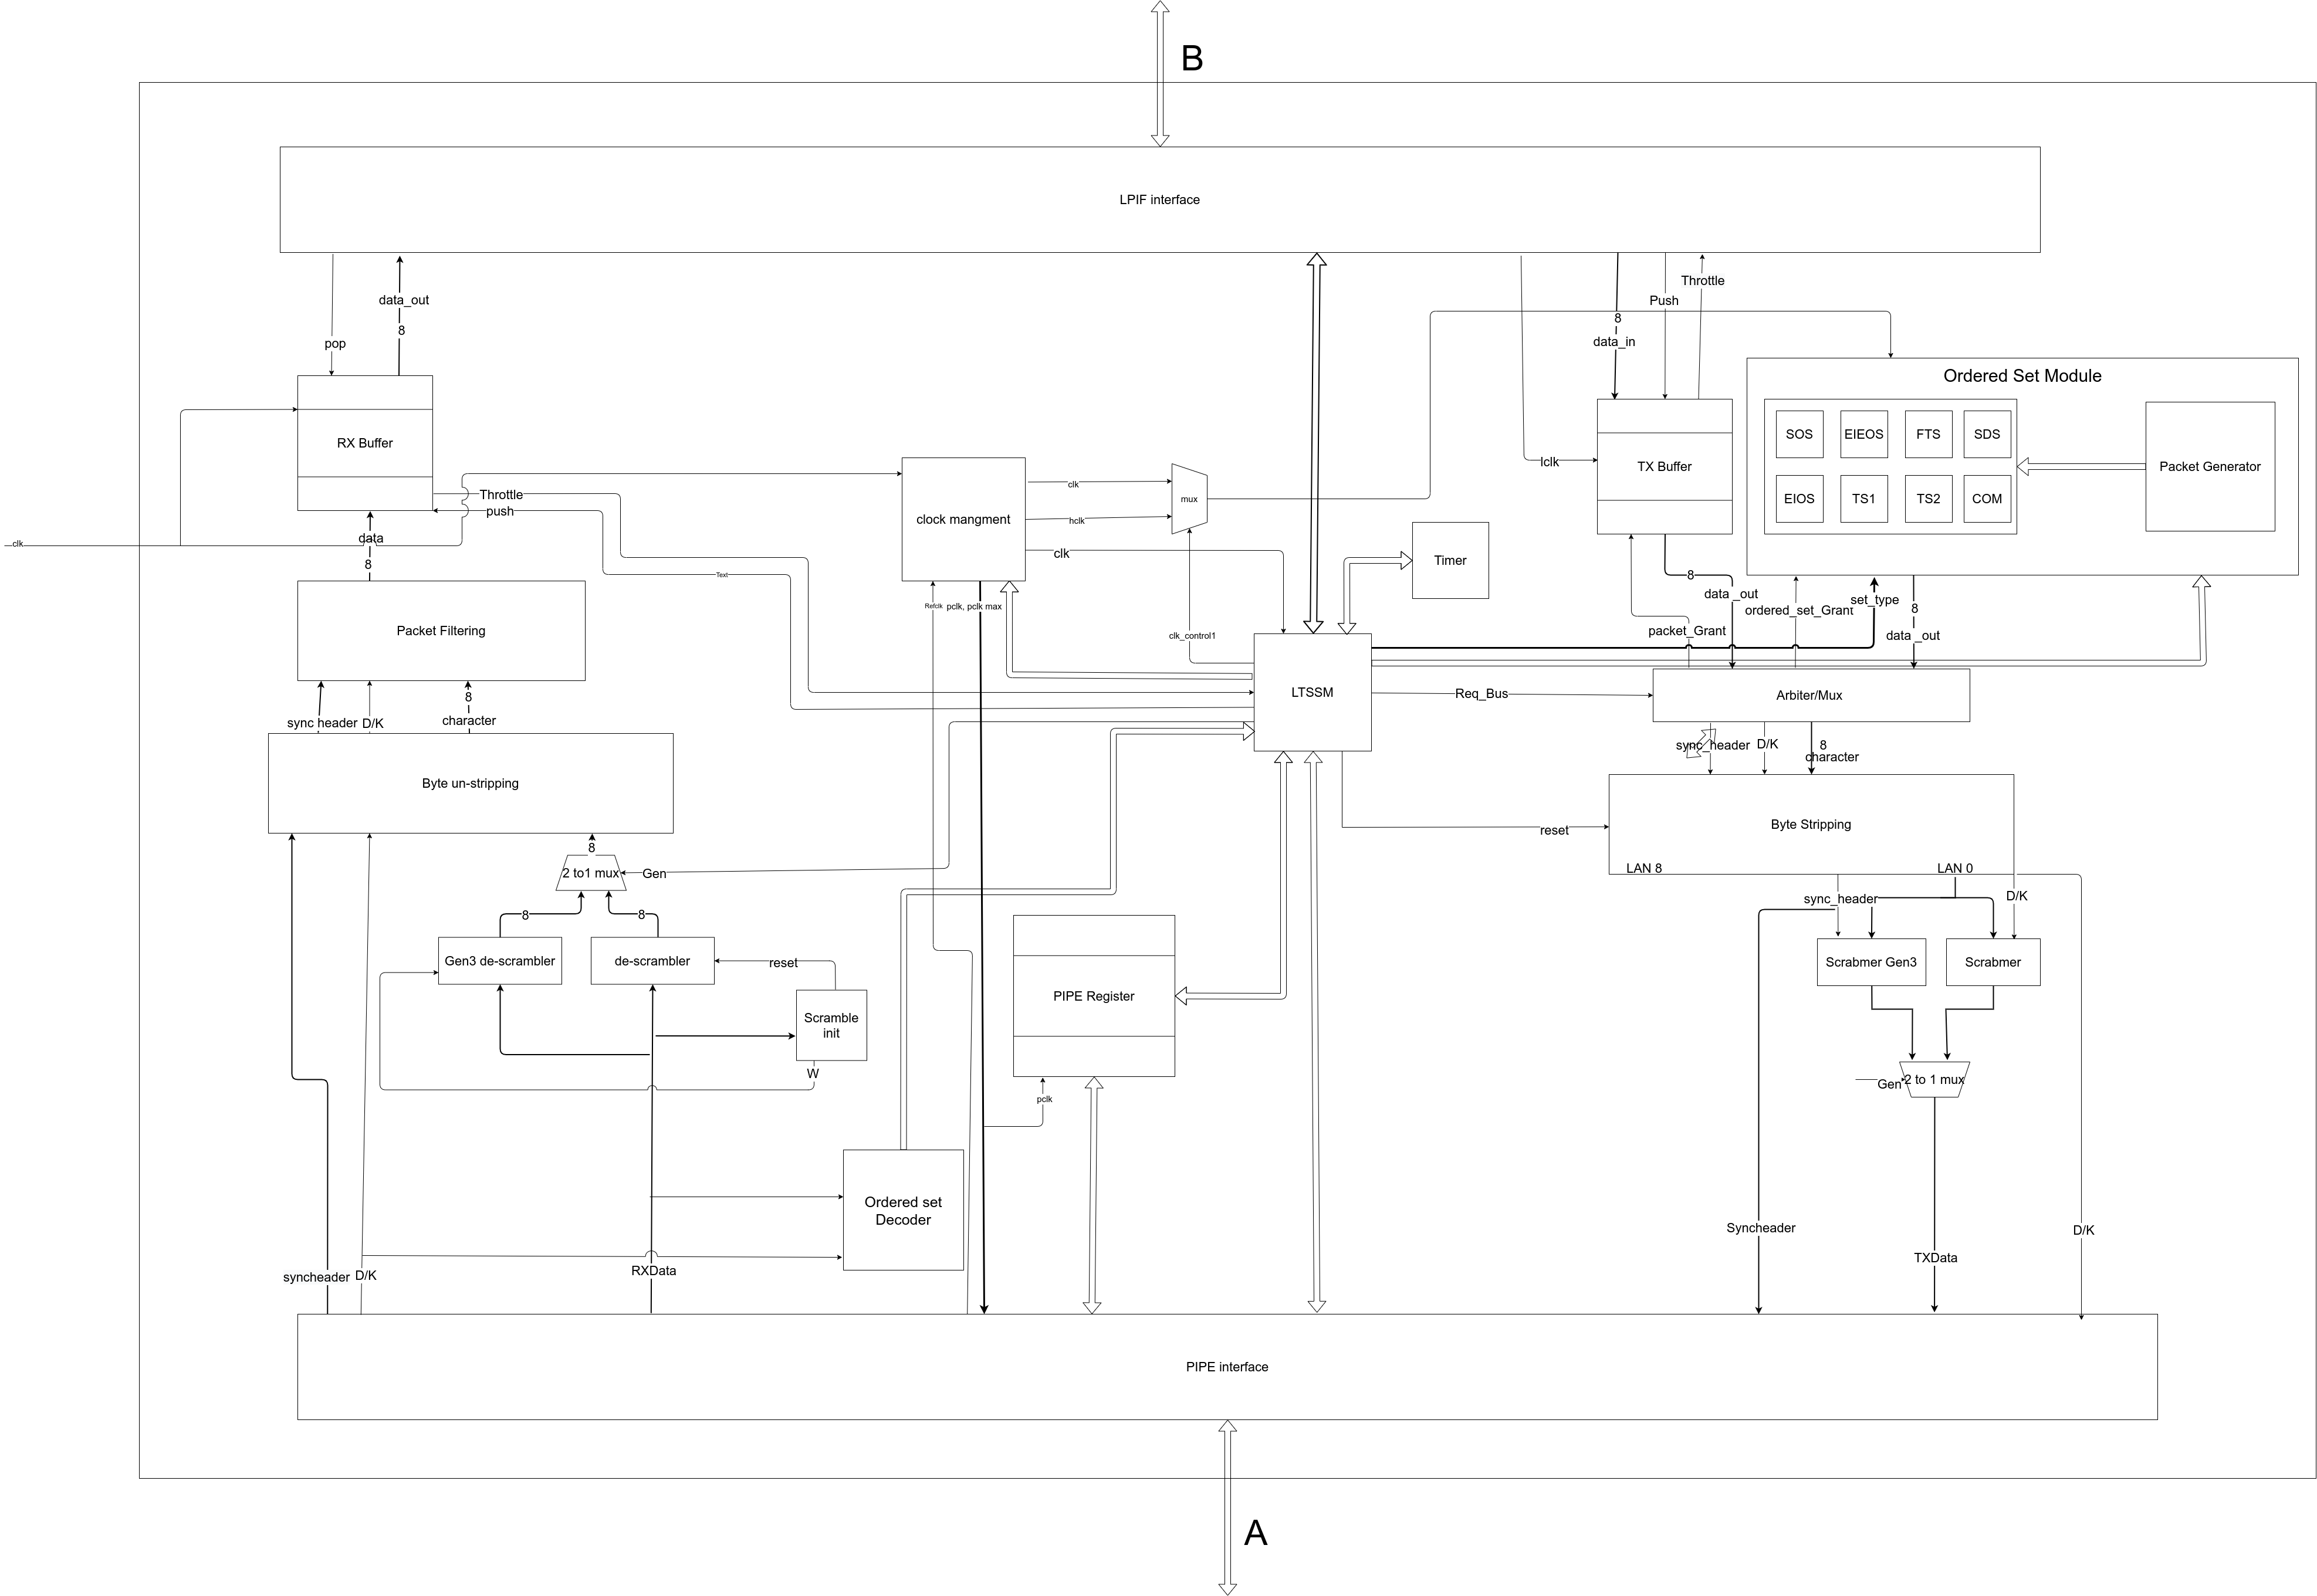
\includegraphics[width=130mm,height=130mm]{images/design-abstract (1).png}
  \caption{MAC Layer Architecture}
  
  \label{fig:arch}
\end{figure}

\subsection{LTSSM}
 \begin{itemize}
     \item Contain Active State Power Management which responsible for power states of the device.
     \item change link width and bit rate. 
     \item send parameters( lane and link number, ....) to Generate Packet module to generate required ordered sets. 
     \item send Req\_Bus signal to arbiter/mux to choose between ordered sets or packet symbol.
     \item choose PCIe generation mode.
 \end{itemize}
 
 \subsection{PIPE Interface}
 It Contains 4 main modules each:
 \begin{itemize}
     \item Rx module \newline
     It receives data from PCS layer in signal RXData and contains Rx related signals(RXsybcheader, RXDatak, .....) see Table \ref{tab:p2}
     \item Tx module \newline
     It tramsites data to PCS layer in signal TXData and contains Tx related signals(TXsybcheader, TXDatak, .....) see Table \ref{tab:p1}
     \item Error handler \newline
     It receives all error signals and generate responde to LTSSM 
    % \item Control unit \newline
    % Encode and Decode message bus \textbf{}
     Note: signal details in Section \ref{sec:1}
     
  \begin{figure}[H]
  \centering
  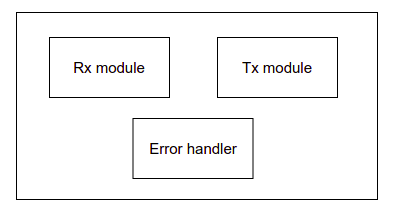
\includegraphics{images/pipe_interface.png}
  \caption{PIPE interface}
  
  \label{fig:pipe}

  
\end{figure}


 \end{itemize}
 
  \subsection{LPIF Interface}
  
  \begin{itemize}
      \item   LPIF Error handler receives all error signals then make some process to send decision to  LPIF ctl 
        \item LPIF ctl control  Txbuffer and Rxbuffer based on error and status signals and send his status to LTSSM to control other modules based on this situation 
  \end{itemize}

  \begin{figure}[H]
  \centering
  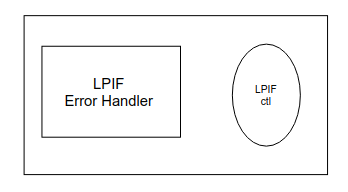
\includegraphics{images/lpif_1.png}
  \caption{LPIF interface}
  
  \label{fig:pipe}
\end{figure}

\subsection{Scrambler init}
\begin{itemize}
    \item COM Detector \newline
    Detect 6 COM symbols to reset scrambler in gen 1,2
    \item SKP Detector \newline
    Detect skp ordered set based on this it sets $W$ signal which next value LFSR is taked as a seed to scrambler gen 3
\begin{figure}[H]
  \centering
  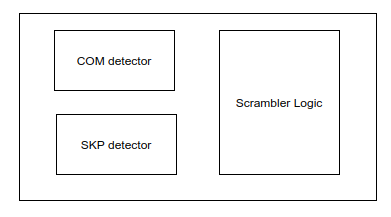
\includegraphics[height=50mm,width=100mm]{images/init.png}
  \caption{Scrambler init}
\end{figure}

\end{itemize}


\subsection{Ordered set and packet Generator module}
\begin{itemize}
    \item Ordered Set module \newline It contains 6 orederd sets end each set has two generation packets. 
\item Packet Generator module \newline It is responsible to  generate gen 3 ordered sets.
\end{itemize}

\begin{figure}[H]
  \centering
  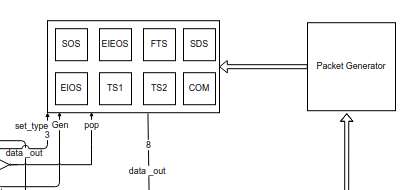
\includegraphics{images/ordered_set.png}
  \caption{Ordered set and packet Generator module}
\end{figure}


% \begin{table}[H]
%     \caption{Input signals for ordered set module}
%     \centering
%   \begin{tabular}{ |m{26mm}|m{60mm}|  }
% \hline
% \rowcolor{Gray}
% \multicolumn{1}{|c|}{\textbf{Name} } 
% & \multicolumn{1}{|c|}{\textbf{Description}}\\
% \hline
%  set\_type  &  choose ordered set type (SOS, EIEOS, ....) \\ \hline 
%   Gen & choose generation of the packet gen 1$\longrightarrow $2 or gen 3$\longrightarrow$5 \\ 
%  \hline 
%  pop & It pops the packet to the bus (data\_out) symbol by symbol until finish \\
%  \hline 


% \end{tabular}
% \end{table}

\subsection{Detailed Design}
\begin{figure}[H]
  \centering
  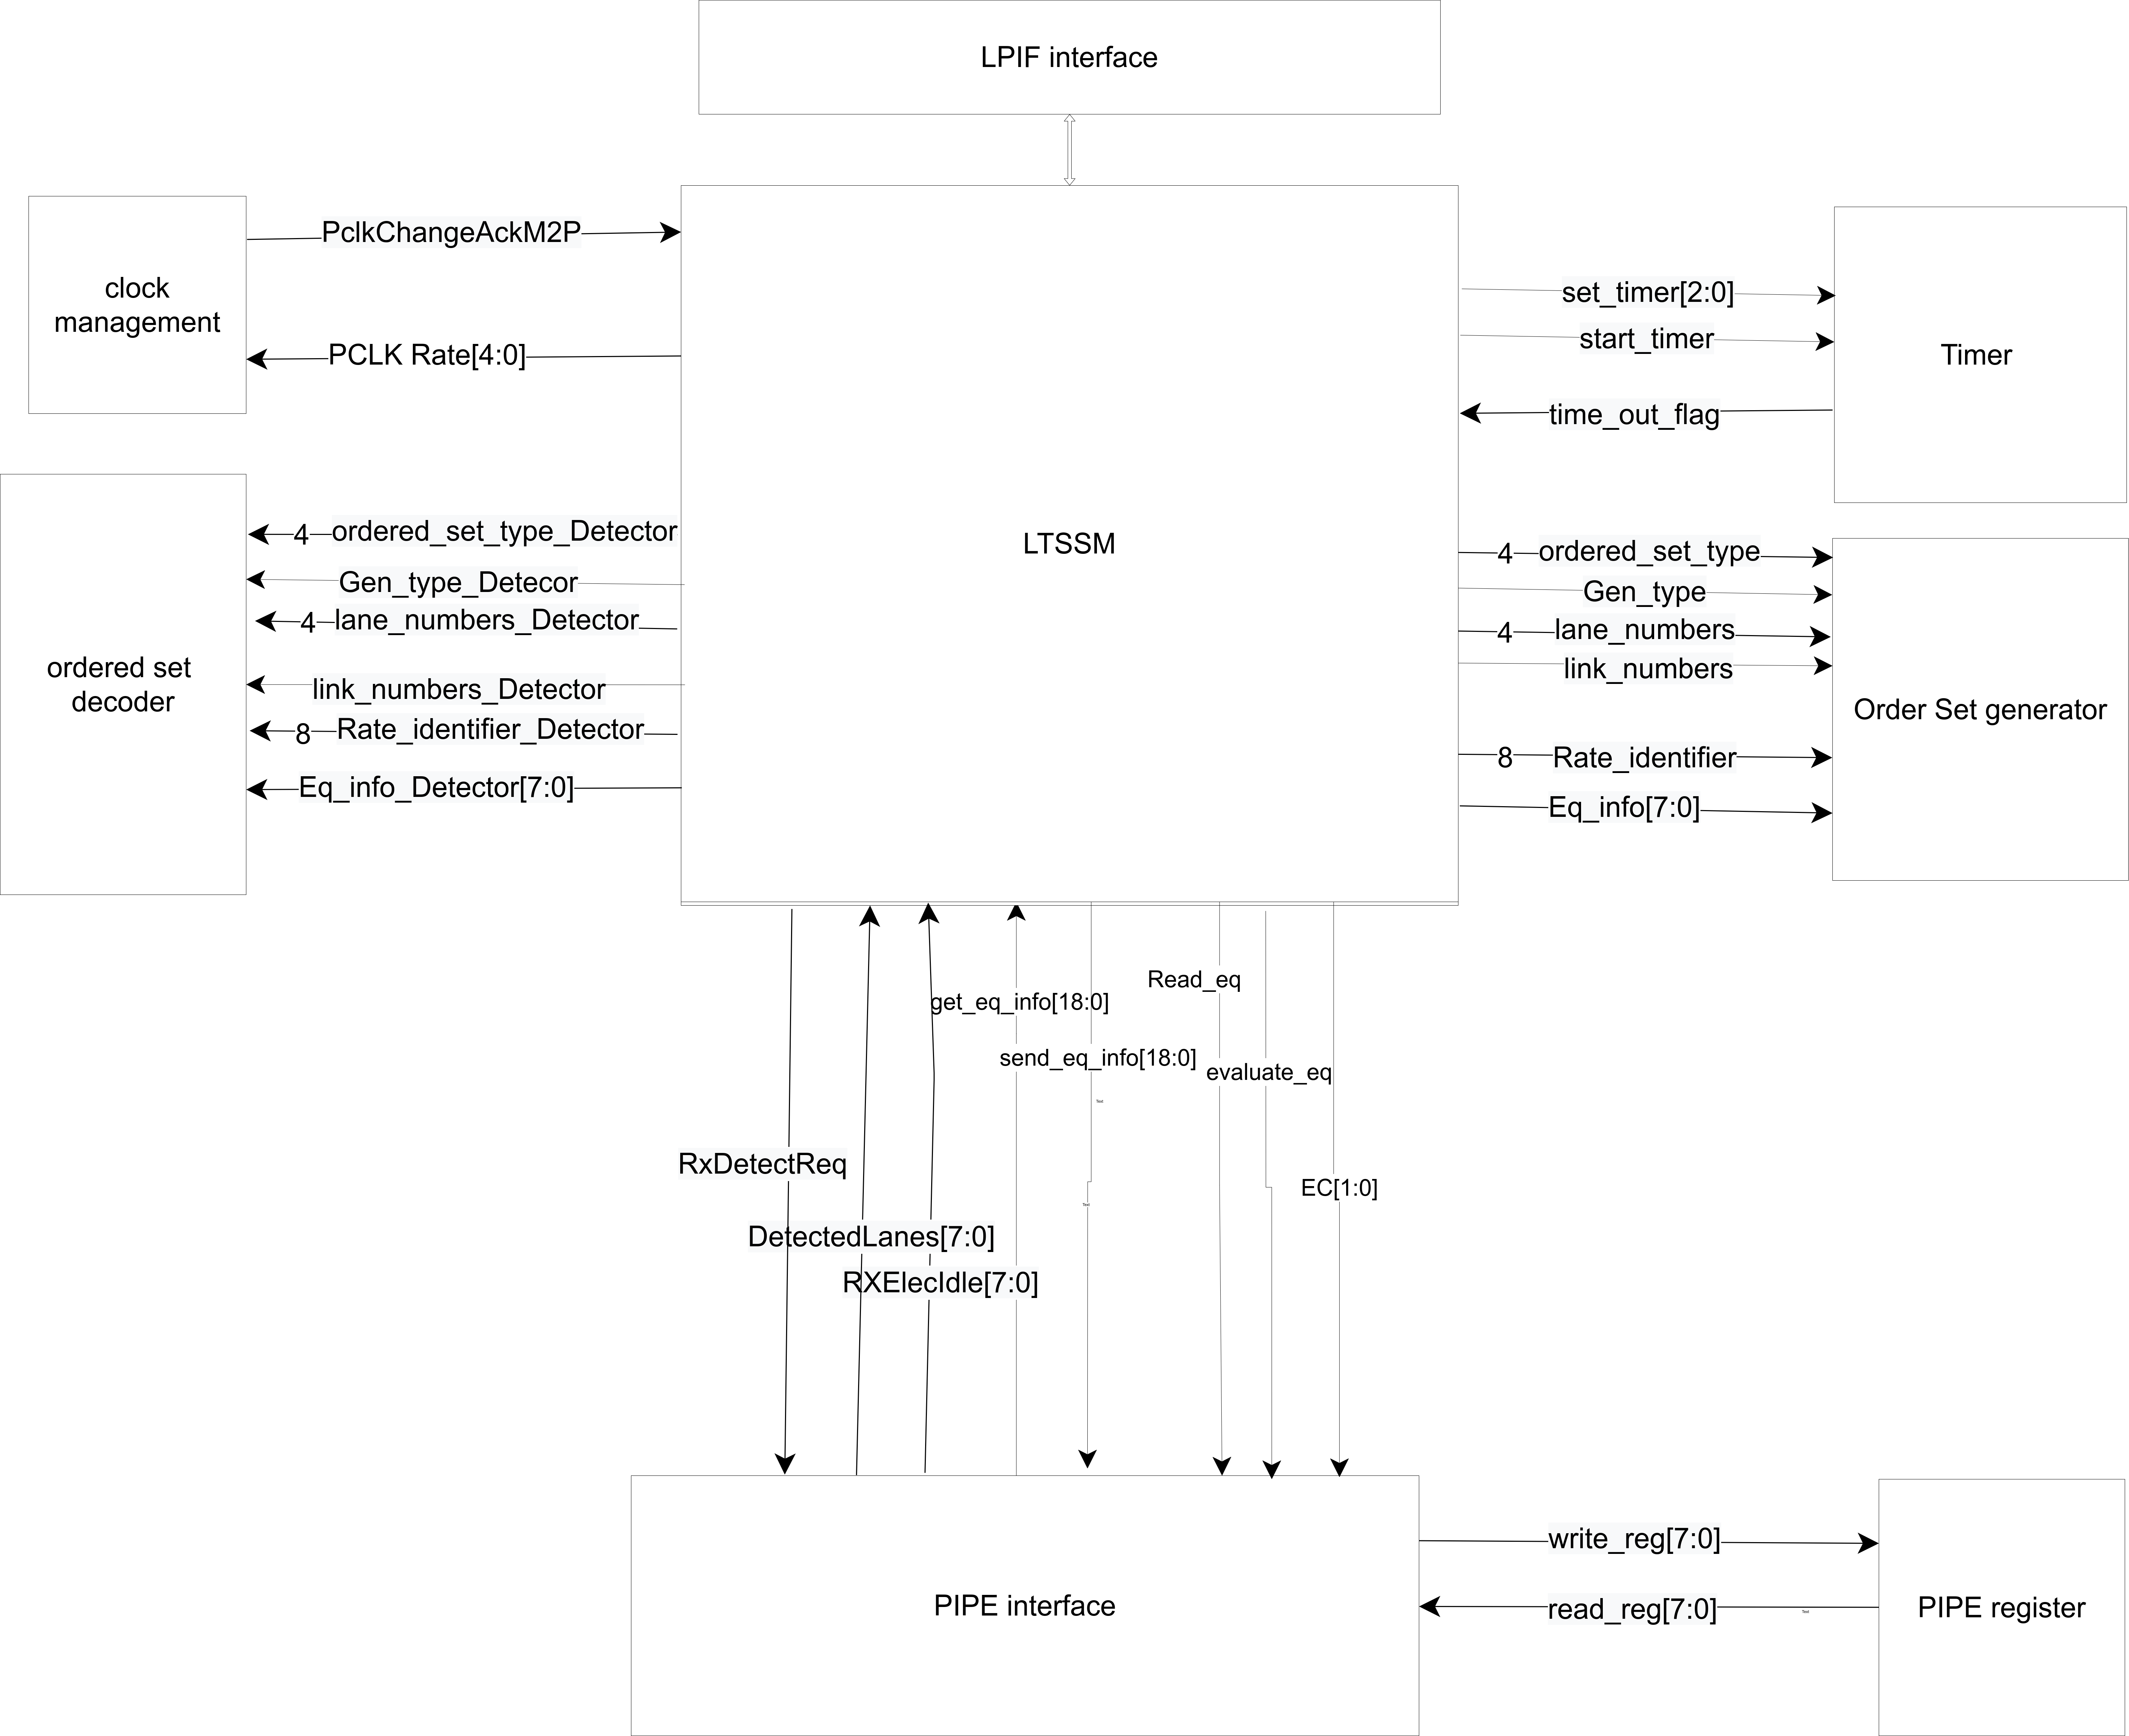
\includegraphics[height=100mm,width=100mm]{images/design-internal_signal.png}
  \caption{LTSSM interfaces with other modules}
\end{figure}
